\documentclass{acm_proc_article-sp}

\usepackage{xspace}
\newcommand{\CEU}{\textsc{C\'{e}u}\xspace}
\newcommand{\code}[1] {{\small{\texttt{#1}}}}

\usepackage{verbatim}
\usepackage{color}
\definecolor{light}{gray}{0.87}
\definecolor{dark}{gray}{0.30}
%\definecolor{light}{rgb}{.90,.90,.90}
\definecolor{darkgreen}{rgb}{0,.50,0}
\definecolor{darkblue}{rgb}{0,0,.50}
\definecolor{darkred}{rgb}{.50,0,0}
\definecolor{darkpur}{rgb}{.50,0,.50}

% \input bnf.tex

\usepackage{listings}
%\usepackage{textcomp}
\lstset{
%columns=fullflexible,
%basicstyle=\ttfamily,
escapeinside={||},
    %mathescape=true,
    language=C, % choose the language of the code
    basicstyle=\fontfamily{pcr}\selectfont\scriptsize\color{black},
    keywordstyle=\color{black}\bfseries, % style for keywords
    numbers=none, % where to put the line-numbers
    numberstyle=\tiny, % the size of the fonts that are used for the line-numbers
    backgroundcolor=\color{light},
    showspaces=false, % show spaces adding particular underscores
    showstringspaces=false, % underline spaces within strings
    showtabs=false, % show tabs within strings adding particular underscores
    %frame=single, % adds a frame around the code
    tabsize=2, % sets default tabsize to 2 spaces
    %rulesepcolor=\color{gray}
    captionpos=b, % sets the caption-position to bottom
    breaklines=false, % sets automatic line breaking
    %breakatwhitespace=false,
    numbersep=2em,
    emph={par,or,hor,do,end,loop,await,emit,input,event,call,with,%
          var,and,then,else,C,return,pure,deterministic,nohold,finalize,%
          class, every, FOREVER, this, spawn, in, pool, watching, until, 
          interface, each, abort, when, signal, PROC, CHAN, SIGNAL, PAR, not,
          bool, data, tag, escape, new, traverse},
    emphstyle={\bfseries},
    commentstyle=\color{dark}\scriptsize,
    %xleftmargin=20pt,
    %xrightmargin=20pt,
    framesep=20pt,
    %upquote=true,
    %aboveskip={1.5\baselineskip},
}

\begin{document}

\title{Reactive Traversal of Recursive Data Types (?!)}
%\subtitle{[Extended Abstract]

\numberofauthors{3}
\author{
\alignauthor
Francisco Sant'Anna \\
    \affaddr{Departamento de Inform\'atica --- PUC-Rio, Brazil} \\
    \email{fsantanna@inf.puc-rio.br}
\alignauthor
Hisham Muhammad \\
    \affaddr{Departamento de Inform\'atica --- PUC-Rio, Brazil} \\
    \email{hisham@inf.puc-rio.br}
\alignauthor
Johnicholas Hines \\
    \affaddr{Affiliation} \\
    \email{email@domain.com}
}

\maketitle
\begin{abstract}
We propose a structured mechanism to traverse recursive data types 
incrementally, in successive reactions to input events.
\code{traverse} is an iterator-like anonymous block that can be invoked 
recursively and suspended at any point, retaining the full state and stack 
frames alive.
\code{traverse} is designed for the synchronous language \CEU, inheriting all 
of its concurrency functionality and safety properties, such as parallel 
compositions with orthogonal abortion, static memory management, and bounded 
reaction time and memory usage.
We discuss three applications in the domains of incremental computation and 
control-oriented DSLs that contain reactive and recursive behavior at the same 
time.

\begin{comment}
MIX OF:
\begin{itemize}
    \item recursive calls to anonymous closures
    \item each instance---many co-routines
\end{itemize}

DESIGNED FOR \CEU:
\begin{itemize}
    \item lexical compositions
    \item static memory management
    \item bounded execution/memory
    \item reactive
    \item mutation
\end{itemize}
\end{comment}

\end{abstract}

\category{D.3.3}{Programming Languages}{Language Constructs and Features}

\terms{Design, Languages}

\keywords{Behavior Trees, Domain Specific Languages, Incremental Computation, 
Logo, Recursive Data Types, Structured Programming, Reactive Programming}

\section{Introduction}

\begin{comment}
All examples have working implementations:

- TODO: compare the real code with the listing

\begin{itemize}
\item label "lst.list":               rebls-15/list/list.ceu
\item label "lst.list.sum":           rebls-15/list/list.ceu
\item label "lst.list.sum.react":     rebls-15/list/list.ceu
%
\item label "lst.bt1":                rebls-15/bts-ceu/btree-1.ceu
\item label "lst.bt1.interpreter":    rebls-15/bts-ceu/btree-1.ceu
\item label "lst.bt1.leaf":           rebls-15/bts-ceu/domain-1.ceu
%
\item label "lst.turtle.dsl":         rebls-15/turtle/turtle-2.ceu
\item label "lst.turtle.interpreter": rebls-15/turtle/turtle-2.ceu
\item label "lst.turtle.queue":       rebls-15/turtle/turtle-7.ceu
%
\item label "lst.gray":               rebls-15/loopless/gray/gray-vec.ceu
\end{itemize}
\end{comment}

\begin{comment}
Difficult because of
    multiple stack frames
    concurrent stack frames
    persistent stack frames (across reactions, with other parts executing)
    static memory management
    mutation of the data structure being traversed
\end{comment}

The facilities offered by a language for constructing data types and values
have a direct impact on the nature of algorithms that programmers of that
language will write. The design of such facilities, on its turn, must take
into account the constraints imposed by the rest of the language. For example,
functional languages aim for referential transparency, and for this reason
they typically present recursive data types as constructors for immutable data
structures. One must then take care when writing algorithms using those
structures to avoid excessive memory copying. A means to do that is to use
data structures that alleviate the lack of random access to components and
in-place modification, such as the ones presented by Okasaki in
\cite{okasaki.purely}.

In this paper, we discuss the design of recursive data types and an associated
control facility for a language developed under a different set of
constraints. \CEU~\cite{ceu.sensys13} is an imperative, concurrent and
reactive language in which the lines of execution, known as \emph{trails},
react all together continuously and in synchronous steps to external stimuli.
Being an imperative language, \CEU features mutable data. At the same time,
however, its design promotes static memory management through lexically-scoped
memory pools, and safety guarantees for concurrent pointer manipulation
through orthogonal abortion~\cite{ceu.mod15}. These features preclude the
availability of general mutable records such as C-style structs with arbitrary
pointers. Recursive data types in \CEU must, therefore, respect the language's
memory management guarantees and their use must cope with the synchronous
concurrency model.

The solution to this problem is twofold, with data and control aspects to it.
For data management, we introduce to the language a \code{data} type construct
with a set of restrictions on instance constructors and assignment semantics
that makes static memory management possible. For handling reactive control,
we propose a structured mechanism to traverse recursive data types
incrementally, in successive reactions to input events. \code{traverse} is an
iterator-like anonymous block that can be invoked recursively and suspended at
any point, retaining the full state and stack frames alive.

Following the presentation of these constructs and their design, we showcase
their use by discussing three applications in the domains of incremental
computation and control-oriented DSLs that contain reactive and recursive
behavior at the same time.

\section{C\'eu constructs}

\begin{comment}
\item adts
\item description
\item expansion: pool / recursive spawn
\item mutation / safety / watching
\end{comment}

\begin{figure}%[t]
\begin{lstlisting}[numbers=left,xleftmargin=3em]
input void RESET;  // declares an external event
var int v = 0;     // variable shared by the trails
par do
   loop do         // 1st trail
      await 1s;
      v = v + 1;
      _printf("v = %d\n", v);
   end
with
   loop do         // 2nd trail
      await RESET;
      v = 0;
   end
end
\end{lstlisting}
\caption{ Introductory example in \CEU.
\label{lst.intro}
}
\end{figure}

In this section, we present the constructs added to \CEU to support recursive
data types with reactive traversal. We begin, though, with a short
introduction to present the general flavor of the language.

The introductory example in Figure~\ref{lst.intro} defines an input event 
\code{RESET} (line 1), a shared variable \code{v} (line 2), and starts two 
trails with the \code{par} construct (lines 3-14): the first (lines 4-8) 
increments variable \code{v} on every second and prints its value on screen; 
the second (lines 10-13) resets \code{v} on every external request to 
\code{RESET}.
\CEU is tightly integrated with \emph{C} and can access libraries of the 
underlying platform directly by prefixing symbols with an underscore (e.g., 
\code{\_printf(<...>)}, in line 7).

In the synchronous model of \CEU, a program reacts to an occurring event 
completely before handling the next.
%
A reaction represents a logical instant in which all trails awaiting the 
occurring event awake and execute, one after the other, until they await again 
or terminate.
%
During a reaction, the environment is invariant and does not interrupt the 
running trails.
If multiple trails react to the same event, the scheduler employs lexical 
order, i.e., the trail that appears first in the source code executes first.
%
For this reason, programs are deterministic even in the presence of side 
effects in concurrent lines of execution.
%
To avoid infinite execution for reactions, \CEU ensures that all loops contain 
\code{await} statements~\cite{ceu.sensys13}.

\subsection{Recursive Data Types}

The \code{data} construct in \CEU provides a safer alternative to C's
\code{struct}, \code{union}, and \code{enum} definitions. A \code{data} entry
declares either a non-recursive structure containing a set of mutable fields
or a tagged union. A tagged union consists of a set of tag declarations, each
of which may be a bare tag or contain mutable fields. If any of the tag
declarations refers to the data type being declared, we have a recursive data
type. In this case, the first tag of the tagged union must be a bare tag, and
it will act as the union's null type: in \CEU, every recursive data type
is an option type.

%%% (Uncomment \input bnf.tex above)
%\begin{figure}[t]
%\begingrammar
%<data> : "data" <id> "with" <dataBody> "end" ";"
%
%<dataBody> : <field>* | <tags>
%
%<tags> : <tag> [ "or" <tags> ]* 
%
%<tag> : "tag" <id> \{ ";" | "with" <field>* "end" \}
%
%<field> : "var" <type> <id> ";"
%
%\endgrammar
%\caption{
%The \code{data} construct in \CEU
%}
%\end{figure}

% rebls-15/list/list.ceu
\begin{figure}[t]
\begin{lstlisting}[numbers=left,xleftmargin=3em]
data List with
   tag NIL;
or
   tag CONS with
      var int  head;
      var List tail;
   end
end

do
   pool List[1] lst1;
   lst1 =new List.CONS(10,
              List.CONS(20,
               List.CONS(30,
                List.NIL()));
   _printf("%d, %d\n", lst1:CONS.head,
                  lst1:CONS.tail:NIL);
      // prints 10, 1
end

do
   pool List[] lst2;
   lst2 =new List.CONS(10,
              List.CONS(20,
               List.CONS(30,
                List.NIL()));
   lst2:CONS.tail =new List.CONS(50, List.NIL());
   _printf("%d\n", lst2:CONS.tail:CONS.head);
      // prints 50 (20 and 30 have been freed)
end
\end{lstlisting}
\caption{
A recursive \code{List} data type definition (lines 1--8) and uses (lines 
10--18 and 20--28).
\label{lst.list}
}
\end{figure}

Figure~\ref{lst.list} illustrates the recursive \code{List} data type,
declared as a tagged union. The first tag, \code{NIL} (line 2), represents
the empty list and is the union's null type. The second tag, \code{CONS},
holds a value in its field \code{head} and a pointer to the rest of the list
in the field \code{tail} (lines 4--7).

All memory allocated by \CEU constructs is managed by lexically-scoped memory
pools. The \code{pool} keyword declares a memory pool of a given size and
a reference to a root object. In line 11, we declare a pool of \code{List}
objects of size 1, identified by root reference \code{lst1},
scoped by the \code{do} block in lines 10--19.
The declaration also implicitly initializes the root to the null tag of the 
associated data type (i.e., \code{List.NIL}).

Then, in lines 12--15, we use the \code{=new} construct, which performs
allocation and assignment: it attempts to dynamically allocate a list of
three elements (using three \code{List.CONS} constructors in the assignment
\emph{r-value}), inferring the destination memory pool based on the 
assignment's \emph{l-value} (i.e. \code{lst1}).

Since the pool has size 1, only the allocation of first element succeeds, with the failed 
allocations returning the null tag for this type (i.e., \code{List.NIL}).
The print command (line 16) outputs ``\texttt{10, 1}'': the \code{head} of the 
first element (the operator \code{`:'} is equivalent to C's \code{`->'}) and 
a true value for the \code{NIL} check of the second element.

In the second block (lines 21--30), we declare the \code{lst2} pool with an
unbounded memory limit (i.e., \code{List[]} in line 22).
Now, the three-element allocation succeeds (lines 23--26).
Then, we mutate the tail of the first element to point to a newly allocated 
element in the same pool, which also succeeds (line 27).
The print command (line 28) outputs ``\texttt{50}'', displaying the \code{head}
of the new second element.
In the moment of the mutation, the old subtree (containing values  ``\texttt{20}''
and  ``\texttt{30}'') is completely removed from memory.
Finally, the end of the block (line 30) deallocates the pool along with all of 
its elements.

%TODO: invalid tag generates runtime error

In \CEU, recursive data types have a number of restrictions.
Given that mutations deallocate whole subtrees, data types cannot represent 
general graphs: they must represent tree-like structures.
Elements in different pools cannot be mixed;
and pointers to subtrees (i.e., weak references) must be observed via the
\code{watching} construct, as they can be invalidated at any time
(to be discussed in Section~\ref{sec.traverse}).

%TODO: what kind of structure updates can be made through weak pointers?

\subsection{Traversing Data Types}
\label{sec.traverse}

\CEU introduces a structured mechanism to traverse data types.
The \code{traverse} construct integrates well with the synchronous execution 
model, supporting nested control compositions, such as \code{await} and all 
\code{par} variations.
It also preserves explicit lexical scopes with static memory management.

% rebls-15/list/list.ceu
\begin{figure}%[t]
\begin{lstlisting}[numbers=left,xleftmargin=3em]
pool List[3] l = new List.CONS(10,
                      List.CONS(20,
                       List.CONS(30,
                        List.NIL())));

var int sum =
   traverse e in l do
      if e:NIL then
         escape 0;
      else
         var int sum_tail = traverse e:CONS.tail;
         escape sum_tail + e:CONS.head;
      end
   end;
_printf("sum = %d\n", sum);
      // prints 60
\end{lstlisting}
%\rule{8.5cm}{0.37pt}
\caption{
Calculating the \emph{sum} of a list.
\label{lst.list.sum}
}
\end{figure}

We begin by showing the flavor of the construct through an example.
The code in Figure~\ref{lst.list.sum} creates a list (lines 1--4) and traverses 
it to calculate the sum of elements (lines 6--15).
The \code{traverse} block (line 7) starts with the element \code{e} pointing to 
the root of the list \code{l}.
The \code{escape} statement (lines 9 and 12) returns a value to be assigned to 
the \code{sum} (line 6).
A \code{NIL} list has \code{sum=0} (lines 8-9).
A \code{CONS} list needs to calculate the \code{sum} of its tail recursively, 
invoking \code{traverse} again (line 11), which will create a nested instance 
of the enclosing \code{traverse} block (lines 7--14), now with \code{e} 
pointing to the \code{e:CONS.tail}.
When used without event control mechanisms, as in this simple example,
a \code{traverse} block is equivalent to an anonymous closure called recursively.

% rebls-15/list/list.ceu
\begin{figure}%[t]
\begin{lstlisting}[numbers=left,xleftmargin=3em]
pool List[] l = <...>;  // 10, 20, 30
var int sum =
   traverse e in l do
      if e:NIL then
         escape 0;
      else
         watching e do
            _printf("me = %d\n", e:CONS.head);
            await 1s;
            var int sum_tail = traverse e:CONS.tail;
            escape sum_tail + e:CONS.head;
         end
         escape 0;
      end
   end;
_printf("sum = %d\n", sum);
\end{lstlisting}
%\rule{8.5cm}{0.37pt}
\caption{
Calculating the \emph{sum} of a list, one element each second.
\label{lst.list.sum.react}
}
\end{figure}
% TODO: react.ceu with mutation

The \code{traverse} construct does not simply amount to an anonymous recursive
block, however. It is designed to take into account the event system and
memory management discipline of the language. As such, it is an abstraction
defined in terms of more fundamental \CEU features: \emph{organisms}, which
are objects with their own parallel trail of execution, akin to Simula
objects; and orthogonal abortion, which handles cancellation of trails
maintaining memory consistency~\cite{ceu.mod15}.

Three aspects make \code{traverse} fundamentally different from an anonymous
recursive function. First, each \code{traverse} call spawns a new anonymous
organism, launching a new parallel trail of execution (as opposed to stacking
a new frame in the current trail). Second, traversal is declared in terms of a
specific memory pool. Therefore, for bounded pools (e.g., \code{List[3] l}),
we can infer at compile time the maximum traversal depth. Third, the execution
body of a \code{traverse} block is implicitly wrapped by a concurrency
construct that watches for mutations of the current node. In practice, this
means that it reacts consistently if another trail of execution modifies the
data structure being traversed.

To illustrate these differences, Figure~\ref{lst.list.sum.react} extends the body
of the previous example with reactive behavior.
For each recursive iteration, \code{traverse} prints the current 
\code{head} (line 8) and awaits 1 second before traversing the \code{tail} 
(lines 9--10).
In \CEU, all accesses to pointers that cross \code{await} statements must be 
protected with \code{watching} blocks~\cite{ceu.mod15}.
This ensures that if side effects occurring in parallel affect the pointed 
object, no code uses stale pointers because the whole block is aborted.
In the example (lines 7--12), if the list is mutated during that 1 second and 
the specific element is removed from memory, we simply ignore the whole subtree 
and return 0.

The \code{traverse} construct allows us to enforce bounded execution time, by
performing a limited number of steps, each of them a separate synchronous
reaction. This can be asserted by verifying that the structure of the
recursive steps converge to the base cases, or simply by using a bounded
memory pools, which allows us to limit the maximum number of steps to the size
of the pool. Enforcing execution limits is an important requirement for
constrained and real-time embedded systems, which is the original application
domain of \CEU~\cite{ceu.sensys13}.

% TODO: abstract fold example?
% TODO: or mention that is not the focus here
% TODO: or mention that abstractions will be used in the applications
\begin{comment}
\begin{figure}%[t]
\begin{lstlisting}[numbers=left,xleftmargin=3em]
class FoldL with
   pool List[]&   l;
   pool Action[]& actions;
   var  int&     acc;
do
   traverse e in l do
      if e:CONS then
         var Action*? a =
            spawn Action(e, acc);
         await *a;
      end
   end
end
\end{lstlisting}
%\rule{8.5cm}{0.37pt}
\caption{
Calculating the \emph{sum} of a list.
\label{lst.sum}
}
\end{figure}
\end{comment}

\section{Applications}

In this section, we present three applications that explore the reactive and 
incremental nature of the \code{traverse} construct.
We start with standard \emph{Behavior Trees} used in video games for AI 
modeling~\cite{TODO}, and extend them with parallel compositions.
Then, we show a \emph{Logo Turtle}~\cite{TODO} that can execute commands in 
parallel (e.g., \code{move} and \code{rotate}) and also incorporates a dynamic 
queue of commands issued concurrently with the running program.
Finally, we implement \emph{Gray code} generation~\cite{TODO} to illustrate how 
\code{traverse} can also be used for more general recursive algorithms without 
an associated data type.

\begin{comment}
How many applications will we present?

\begin{itemize}
    \item behavior trees (DSL)
    \item logo turtle (DSL)
    \item turtle stream (incremental)
    \item gray code gen (incremental)
\end{itemize}

I suggest gray code as the last one because it does not use a data type.
We could show as an example of flexibility of traverse.
BTs before turtle because they are simpler and because the stream example is 
the most complex and should follow the logo turtle.
\end{comment}

\subsection{Behavior Trees}

The term \emph{Behavior Trees} denotes a family of DSLs used for Game 
AI~\cite{TODO}.
The term is loose, because different games use different languages,
but generally it indicates an interpreted domain-specific language
for creature behavior that includes at least sequence and selection combinators,
and which are ``ticked'' periodically~\cite{TODO}.

%\subsubsection{A Standard Behavior Tree}

The semantics of the sequence combinator can be understood as short-circuit evaluation of a conjunction;
the \code{SEQ} node ticks its left subtree until it finishes,
and if it finishes successfully, ticks its right subtree until it finishes.
The semantics of the selection combinator can be understood as short-circuit evaluation of an alternation;
the \code{SEL} node ticks its left subtree until it finishes,
and if it did not finish successfully, ticks its right subtree until it finishes.

This skeleton, augmented with leaves that test properties, set properties, perform animations and sounds,
and other custom combinators, can be preferable to finite state machines (hierarchical, augmented, or otherwise) for authoring Game AI.

% rebls-15/bts-ceu/btree-1.ceu
\begin{figure}%[t]
\begin{lstlisting}[numbers=left,xleftmargin=3em]
data BTree with
   tag NIL;
or
   tag SEQ with
      var BTree first;
      var BTree second;
   end
or
   tag SEL with
      var BTree first;
      var BTree second;
   end
or
   tag LEAF with
      var Leaf leaf;
   end
end

\end{lstlisting}
%\rule{8.5cm}{0.37pt}
\caption{ A standard behavior tree with \emph{sequence} and \emph{selector}
          composite nodes.
\label{lst.bt1}
}
\end{figure}

% rebls-15/bts-ceu/btree-1.ceu
\begin{figure}%[t]
\begin{lstlisting}[numbers=left,xleftmargin=3em]
class BTreeInterpreter with
   pool BTree[]& btree;
do
   var int ret =
      traverse t in btree do
         if t:SEQ then
             var int ok = traverse t:SEQ.first;
             if ok == 0 then
                 escape ok;
             end
             ok = traverse t:SEQ.second;
             escape ok;
         else/if t:SEL then
             var int ok = traverse t:SEL.first;
             if ok != 0 then
                 escape ok;
             end
             ok = traverse t:SEL.second;
             escape ok;
         else/if t:LEAF then
            var int ret =
                do LeafHandler(t:LEAF.leaf);
            escape ret;
         end
      end;
   escape ret;
end

pool BTree[] btree =
    new BTree.SELECTOR(
        BTree.SEQ(
            BTree.LEAF(Leaf.SENSEONTABLE(3)),
            BTree.SEQ(
                BTree.LEAF(Leaf.MOVEBLOCKTOBLOCK(2, 3, 1)),
                BTree.LEAF(Leaf.MOVEFROMTABLE(3, 2))
            )
        ),
        BTree.SEQ(
            BTree.LEAF(Leaf.MOVETOTABLE(3, 2)),
            BTree.SEQ(
                BTree.LEAF(Leaf.MOVEFROMTABLE(2, 1)),
                BTree.LEAF(Leaf.MOVEFROMTABLE(3, 2))
            )
        )
    );

var int ret = do BTreeTraverse(btree);

_printf("ret = %d\n", ret);     // prints "3"
\end{lstlisting}
%\rule{8.5cm}{0.37pt}
\caption{ A straightforward interpreter for the standard behavior tree of 
          Figure~\ref{lst.bt1} and a blocksworld tree to execute.
\label{lst.bt1.interpreter}
}
\end{figure}

%% rebls-15/bts-ceu/domain-1.ceu
%\begin{figure}%[t]
%\begin{lstlisting}[numbers=left,xleftmargin=3em]
%class LeafHandler with
%   var Leaf& leaf;
%do
%   // TODO: what to show here?
%   escape leaf.v;
%end
%\end{lstlisting}
%%\rule{8.5cm}{0.37pt}
%\caption{ A leaf node with complex behavior.
%\label{lst.bt1.leaf}
%}
%\end{figure}

%\subsubsection{Parallel Behavior Tree}

Ceu's parallel features make implementing a parallel combinator for behavior 
trees much easier.

\begin{comment}
Most "standard" BTs I found have these "sequence" and "selector" composite 
nodes.
I thought about starting with this one and maybe expanding it with a 
"parallel/or" further.

Two things to discuss:
(1) how the implementation of the interpreter is straightforward;
(2) that leaf nodes are not restricted to a "tick" callback and can actually 
execute arbitrary code in \CEU.
\end{comment}

\subsection{Logo Turtle}

Our second example is an interpreter for a simple variant of the classic Logo
turtle-graphics interpreter \cite{papert.logo}, which extends the Logo
paradigm with a \CEU-like parallel execution construct. In our variant, we can
instruct the turtle to move and rotate in parallel, tracing curves. We declare
a data type which defines our abstract syntax, with each tag representing one
of the supported Logo commands. A tree of nodes represents a program, and the
interpreter is implemented as a traversal of this tree. The aim of this
example is to demonstrate parallel traversal.
% TODO: check if BTs will also do par traversal

Figure~\ref{lst.turtle.dsl} presents the data type \code{Command}, which
specifies the abstract syntax of our Logo variant. As in traditional Logo,
commands can be listed in sequence to be executed one after the other
(represented through a chain of \code{SEQ} nodes), and commands can be
repeated a number of times (denoted through a \code{REPEAT} node). Our variant
includes \code{MOVE} and \code{ROTATE} nodes to move the turtle, but these are
specified differently from traditional Logo: here, they take as arguments the
speed at which they should affect the turtle. For example, a
\code{Command.MOVE(50)} node directs the turtle to move at the speed of 50
pixels per second, indefinitely. The only way to make the turtle stop moving
or rotating is through two \CEU-like extensions added to our Logo variant:
\code{AWAIT} and \code{PAROR}. \code{AWAIT} simply awaits a given number of
milliseconds. \code{PAROR}, modeled after the \CEU construct \code{par/or},
launches two commands in parallel, and aborts both of them as soon as one of
them finishes. For example, the following construct would make the turtle move
along a semicircle:

\begin{verbatim}
   Command.PAROR(
      Command.AWAIT(1000),
      Command.PAROR(
         Command.MOVE(50),
         Command.ROTATE(180)))
\end{verbatim}

\begin{comment}
The turtle has three attributes:
    a location
    an orientation
    a pen, itself having attributes such as color, width, and up versus down.
The turtle moves with commands that are relative to its own position, such as 
"move forward 10 spaces" and "turn left 90 degrees". The pen carried by the 
turtle can also be controlled, by enabling it, setting its color, or setting 
its width. A student could understand (and predict and reason about) the 
turtle's motion by imagining what they would do if they were the turtle.  
Seymour Papert called this "body syntonic" reasoning.
From these building blocks one can build more complex shapes like squares, 
triangles, circles and other composite figures. Combined with control flow, 
procedures, and recursion, the idea of turtle graphics is also useful in a 
Lindenmayer system for generating fractals.
Turtle geometry is also sometimes used in graphics environments as an 
alternative to a strictly coordinate-addressed graphics system.
\end{comment}

% rebls-15/turtle/turtle-2.ceu
\begin{figure}%[t]
\begin{lstlisting}[numbers=left,xleftmargin=3em]
data Command with
   tag NOTHING;
or
   tag SEQ with
      var Command one;
      var Command two;
   end
or
   tag REPEAT with
      var int     times;
      var Command command;
   end
or
   tag MOVE with
      var int pixels;
   end
or
   tag ROTATE with
      var int angle;
   end
or
   tag AWAIT with
      var int ms;
   end
or
   tag PAROR with
      var Command one;
      var Command two;
   end
end
\end{lstlisting}
%\rule{8.5cm}{0.37pt}
\caption{ DSL for a Logo turtle.
\label{lst.turtle.dsl}
}
\end{figure}

%% rebls-15/turtle/turtle-2.ceu
%\begin{figure}%[t]
%\begin{lstlisting}[numbers=left,xleftmargin=3em]
%data Command with
%   tag NOTHING;
%or
%   tag SEQ    with var Command one, two; end
%or
%   tag REPEAT with var int times;
%                   var Command command;  end
%or
%   tag MOVE   with var int pixels;       end
%or
%   tag ROTATE with var int angle;        end
%or
%   tag AWAIT  with var int ms;           end
%or
%   tag PAROR  with var Command one, two; end
%end
%\end{lstlisting}
%%\rule{8.5cm}{0.37pt}
%\caption{ DSL for a Logo turtle.
%\label{lst.turtle.dsl}
%}
%\end{figure}

Figure~\ref{lst.turtle.interpreter} depicts the interpreter. It is implemented
as the \code{Interpreter} organism (declared with the \code{class} keyword).
It holds as attributes a reference to the AST of commands (\code{cmds}, line 2)
and a reference to a \code{Turtle} object which implements the UI. The
execution body of the organism contains the \code{traverse} construct which
runs the interpreter (lines 5--35).

We have then a test for each kind of tag in the data type. In lines 7--9,
\code{SEQ} is handled by traversing each of its child commands, in sequence:
the second invocation of \code{traverse} in that block (line 9) only runs
after the first one (line 8) finishes. In lines 11--14, \code{REPEAT} is
handled by traversing its command the specified number of times.

\code{MOVE} is handled in lines 16--18 by spawning a new organism called
\code{TurtleMove}, which launches a separate trail of execution. The
implementation of \code{TurtleMove} (not shown) updates the coordinates of the
\code{turtle} instance it got as a parameter in its constructor. The
implementation of \code{ROTATE} (lines 20--22) is similar.

In lines 24--25, \code{AWAIT} is implemented by simply causing the current
trail of execution of the interpreter to await the given amount of time.
Finally, \code{PAROR} (lines 27--32) uses the \code{par/or} construct
to traverse both subcommands at the same time. As per the semantics of
\code{par/or}, as soon as one of the subtrees terminate its execution,
the other one will be aborted.

Note that the entire interpreter block is surrounded by a \code{watching}
construct (line 6). The \CEU compiler enforces the presence of a guard, 
due to the use of the \code{cmd} pointer in code that spans multiple
reactions. This ensures clean abortion in case the AST being interpreted
is mutated by code running in another trail.

% rebls-15/turtle/turtle-7.ceu
\begin{figure}%[t]
\begin{lstlisting}[numbers=left,xleftmargin=3em]
class Interpreter with
   pool Command[]* cmds;
   var   Turtle&   turtle;
do
   traverse cmd in cmds do
      watching cmd do
         if cmd:SEQ then
            traverse cmd:SEQ.one;
            traverse cmd:SEQ.two;

         else/if cmd:REPEAT then
            loop i in cmd:REPEAT.times do
               traverse cmd:REPEAT.command;
            end

         else/if cmd:MOVE then
            do TurtleMove(turtle,
                          cmd:MOVE.pixels);

         else/if cmd:ROTATE then
            do TurtleRotate(turtle,
                            cmd:ROTATE.angle);

         else/if cmd:AWAIT then
            await (cmd:AWAIT.ms) ms;

         else/if cmd:PAROR then
            par/or do
               traverse cmd:PAROR.one;
            with
               traverse cmd:PAROR.two;
            end
         end
      end
   end
end
\end{lstlisting}
%\rule{8.5cm}{0.37pt}
\caption{ The turtle interpreter.
\label{lst.turtle.interpreter}
}
\end{figure}

\subsubsection{Enqueuing Commands}
\label{sub.enqueuing}

All examples so far create a fixed tree that does not vary during traversal.
%
Figure~\ref{lst.turtle.queue} extends the Turtle application with a queue of 
pending commands to execute after the running commands terminate.

We define a new \code{Queue} data type in (\emph{CODE-1}):
\code{ROOT} has a \code{running} subtree with the running commands, a 
\code{waiting} queue of pending commands to execute, and a \code{tmp} node that 
allows in-place manipulation of the tree.
Given that all newly allocated nodes must reside in a pool, the \code{tmp} node 
represents a pointer TODO.
\code{ITEM} represents a queue item and contains a \code{cmd} subtree with the 
command to execute, and a \code{prv} queue item pointing to an older item that 
should execute first (i.e., the queue is in reverse order).
%
We define a new \code{Queue} data type in \emph{CODE-1}:
The tag \code{ROOT} has a \code{runnning} subtree with the running commands, a 
\code{waiting} queue of pending commands to execute afterwards, and a 
\code{tmp} node to allows in-place manipulation of the tree (to be discussed 
further).
%
The \code{ITEM} tag represents a queue item and contains a \code{cmds} subtree 
with the commands to execute, and a \code{prv} queue item pointing to an older 
item that should execute first (i.e., the queue is in reverse order).
%
As Figure~\ref{fig.queue-1} illustrates, an queue instance should have a single 
\code{ROOT} node with linked lists of \code{ITEM} nodes in the \code{running} 
and \code{waiting} fields.
Except on command creation, the \code{tmp} field is always \code{NIL}.

The \code{queue} traversal in \emph{CODE-2} handles the data type tags 
\code{ROOT} (lines 3--16) and \code{ITEM} (lines 17--22).
%
The \code{ROOT} traversal is a continuous \code{loop} that executes the 
\code{running} subtree and swaps it on termination with the \code{waiting} 
queue.
The \code{par/and} (lines 5--9) ensures that that the swap only occurs after 
the current \code{running} commands terminate (line 6) \emph{and} something 
mutates the \code{waiting} subtree (line 8), meaning that the queue is not 
empty.
The swapping process (lines 10--16) is illustrated in Figure~\ref{fig.queue-2}:
%
\begin{enumerate}
\item We assign the \code{waiting} subtree to the \code{running} field, 
releasing the old subtree (lines 10--11).
\item The \code{waiting} field is automatically set to the \code{NIL} base case 
of the \code{Queue} data type (lines 10--11).
\item We assign a new neutral item to the \code{waiting} queue (lines 12--15).
\end{enumerate}
%
After the swapping process, the \code{loop} restarts and traverses the new 
\code{running} commands.
%
The \code{ITEM} traversal is straightforward:
first we traverse the previous item (line 4), and then we reuse the 
\code{Interpreter} class of Figure~\ref{lst.turtle.interpreter} to traverse the 
commands.

Finally, the \code{every} loop in \emph{CODE-3} reacts to each occurrence of 
the external input event \code{ENQUEUE} (line 1), accepting \emph{move} and 
\emph{rotate} string commands with an associated velocity and time.
The code to enqueue a \emph{move} command (lines 3--15), which is analogous to 
to a \emph{rotate} command (hidden in lines 16--17), is illustrated in 
Figure~\ref{fig.queue-3}:
%
\begin{enumerate}
\item We assign a new neutral \code{ITEM} containing another \code{ITEM} with 
the requested \emph{move} command to the \code{tmp} field.
\item We skip the neutral \code{ITEM} in the root of the \code{waiting} field 
and assign the \code{prv} field (containing the \code{ITEM} with all enqueued 
commands) to the \code{tmp} tail, skipping both the neutral and its nested 
\code{ITEM}.
\item Now, the

The untouched neutral item in the root of the \code{waiting} field ke

and assign to the \code{prv} field of the \code{ITEM} containing the new

The \code{waiting} field is automatically set to the \code{NIL} base case of 
the \code{Queue} data type (lines 10--11).
The neutral item in the root of the \code{waiting} field.
\item We assign a new neutral item to the \code{waiting} queue (lines 12--15).
\end{enumerate}
%
The behavior for XXX is analogous (hidden in lines XX--YY).

- TODO: modularization of data type and travesal

\begin{figure*}%[t]
\begin{minipage}[t]{0.20\linewidth}
\begin{lstlisting}[title=CODE-1: The \code{Queue} data type]
data Queue with
  tag NIL;
or
  tag ROOT with
    var Queue running;
    var Queue waiting;
    var Queue tmp;
  end
or
  tag ITEM with
    var Command cmds;
    var Queue   prv;
  end
end










.
\end{lstlisting}
\end{minipage}
%
\begin{minipage}[t]{0.36\linewidth}
\begin{lstlisting}[numbers=left,xleftmargin=3.5em,title=CODE-2: Queue traversal]
traverse qu in queue do
  watching qu do
    if qu:ROOT then
      loop do
        par/and do
          traverse qu:ROOT.running;
        with
          await qu:ROOT.waiting;
        end
        qu:ROOT.running =
          qu:ROOT.waiting;
        qu:ROOT.waiting =
          new Queue.ITEM(
               Command.NOTHING(),
               Queue.NIL());
      end
    else/if qu:ITEM then
      traverse qu:ITEM.prv;
      do Interpreter with
        this.turtle = turtle;
        this.cmds   = qu:ITEM.cmds;
      end;
    end
  end
end
\end{lstlisting}
\end{minipage}
%
\begin{minipage}[t]{0.39\linewidth}
\begin{lstlisting}[numbers=left,xleftmargin=3.5em,title=CODE-3: Command enqueuing]
input (char*,int,int) ENQUEUE;
every (cmd,vel,time) in ENQUEUE do
  if _strcmp(cmd,"move")==0 then
    queue.ROOT.tmp =
      new Queue.ITEM(
           Command.PAROR(
            Command.MOVE(vel),
             Command.AWAIT(time)),
            Queue.NIL());
  else/if _strcmp(cmd,"rotate")==0 then
    <...>
  end
  queue.ROOT.tmp.ITEM.prv =
    queue.ROOT.waiting.ITEM.prv;
  queue.ROOT.waiting = queue.ROOT.tmp;
end








.
\end{lstlisting}
\end{minipage}
%
%\rule{17.5cm}{0.37pt}
\caption{ Queue extension for the Turtle DSL of
          Figures~\ref{lst.turtle.dsl}~and~\ref{lst.turtle.interpreter}.
\label{lst.turtle.queue}
}
\end{figure*}

\begin{figure}%[t]
\centering
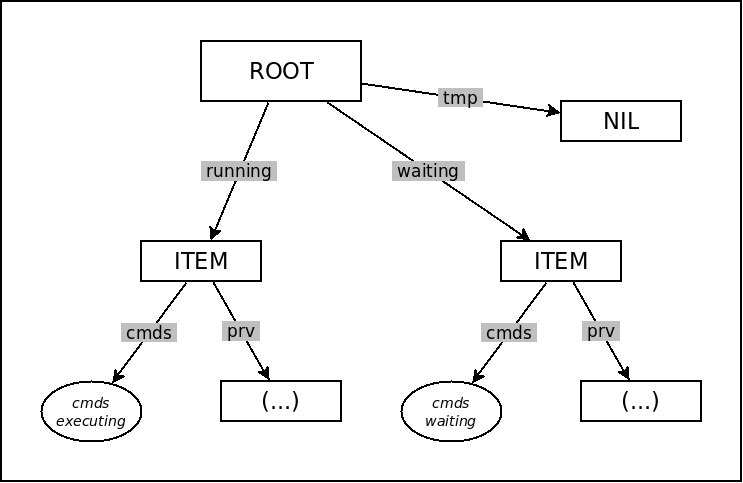
\includegraphics[scale=0.25]{queue-1.png}
\caption{
Structure of a queue of turtle commands.
\label{fig.queue-1}
}
\end{figure}

\begin{figure*}%[t]
\begin{minipage}[t]{0.33\linewidth}
\centering
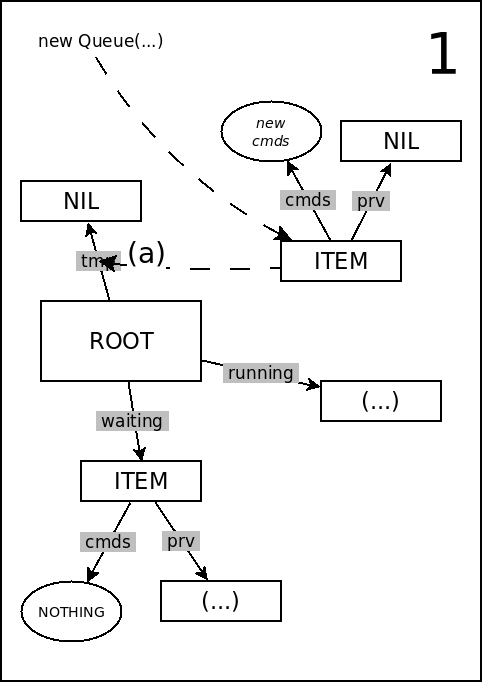
\includegraphics[scale=0.20]{queue-21.png}
\end{minipage}
\begin{minipage}[t]{0.33\linewidth}
\centering
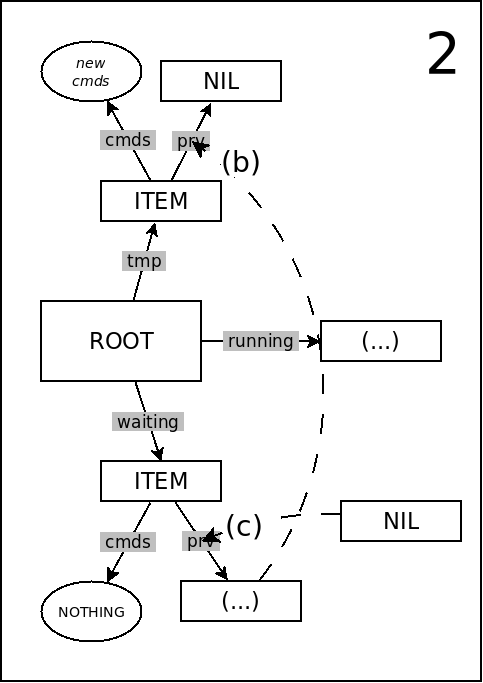
\includegraphics[scale=0.20]{queue-22.png}
\end{minipage}
\begin{minipage}[t]{0.33\linewidth}
\centering
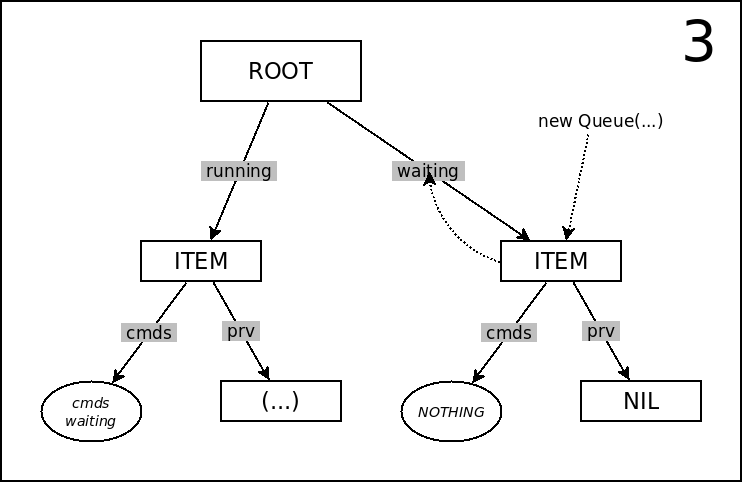
\includegraphics[scale=0.20]{queue-23.png}
\end{minipage}
\caption{
Swapping \code{waiting} and \code{running} commands.
\label{fig.queue-2}
}
\end{figure*}

\begin{figure*}%[t]
\begin{minipage}[t]{0.33\linewidth}
\centering
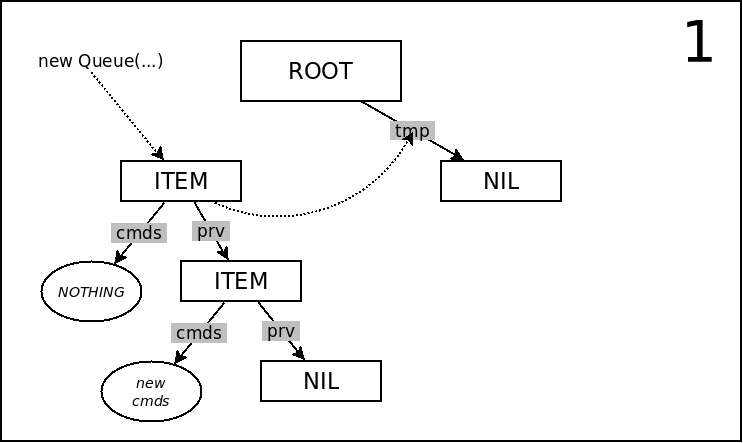
\includegraphics[scale=0.20]{queue-31.png}
\end{minipage}
\begin{minipage}[t]{0.33\linewidth}
\centering
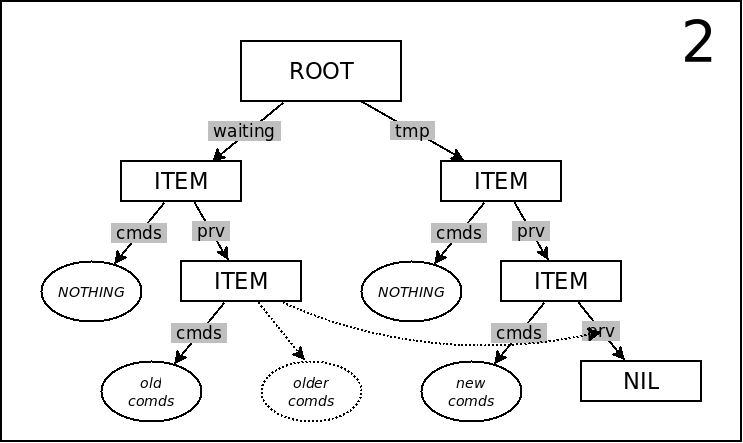
\includegraphics[scale=0.20]{queue-32.png}
\end{minipage}
\begin{minipage}[t]{0.33\linewidth}
\centering
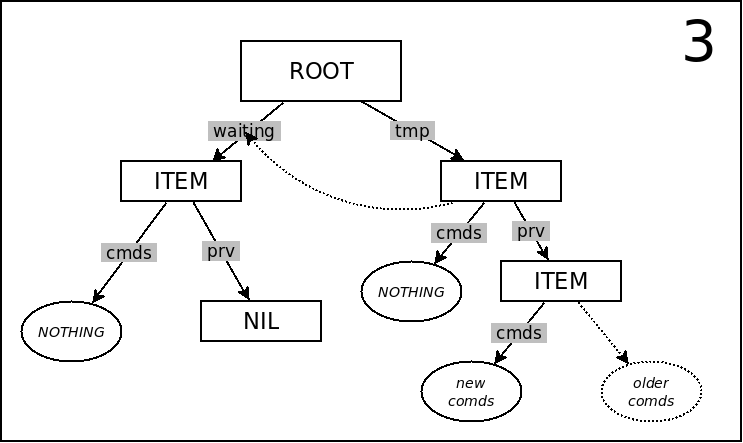
\includegraphics[scale=0.20]{queue-33.png}
\end{minipage}
\caption{
TODO
\label{fig.queue-3}
}
\end{figure*}

\subsection{Gray Code Generation}

% rebls-15/loopless/gray/gray-vec.ceu
\begin{figure}%[t]
\begin{lstlisting}[numbers=left,xleftmargin=3em]
var int[4] bits = [0, 0, 0, 0];

par/or do
   every VISIT do
      _printf("( ");
      loop i in $$bits do // $$ is the array size
         _printf("%d ", bits[i]);
      end
      _printf(")\n");
   end
with
   traverse idx in [$$bits] do
      if idx == $$bits then
         await NEXT;
      else
         traverse idx + 1;
         bits[idx] = 1 - bits[idx];
         traverse idx + 1;
      end
   end
end
\end{lstlisting}
%\rule{8.5cm}{0.37pt}
\caption{ Generator for 4-bit Gray code.
\label{lst.gray}
}
\end{figure}



\section{Related Work}

...

\begin{comment}
What to compare against???

Found this: http://arxiv.org/pdf/1104.2293.pdf
Follow the references.
\end{comment}

\section{Conclusion}

We presented a new construct for traversing recursive data types
incrementally, in the context of \CEU, an imperative reactive language with
synchronous concurrency. The \code{traverse} construct encapsulates an idiom
for performing recursive traversal by handling each step as a separate trail
of execution. This allows parallel traversal using the language's concurrency
features, while maintaining its safety properties.

This kind of traversal can be performed in \CEU through the use of organisms
(pooled objects which launch their own execution trails) and orthogonal
abortion via the \code{watching} construct. Combining these features to
traverse a recursive data structure correctly, however, is not straightforward.
Recursing in a way such that parallel constructs can be composed requires each
step of the recursion to be a new execution trail. Ensuring that the traversal
will not execute on a stale subtree in case the structure is modified requires
the nodes to be watched in order to perform abortions. Additionally, by
presenting a control construct that is tied to a data structure, we can ensure
bounded execution time, in line with the \CEU philosophy. By dealing with these
concerns internally in the \code{traverse} statement, we make reactive
traversal as easy to perform correctly as a recursive function call.

%TODO: mention/review other examples

\begin{comment}
Difficult because of
    multiple stack frames
    concurrent stack frames
    persistent stack frames (across reactions, with other parts executing)
    -DONE- static memory management
    -DONE- mutation of the data structure being traversed
\end{comment}

In the current implementation of recursive data types in \CEU, we impose
restrictions to the kinds of structures that can be represented. The
requirement of a tree hierarchy of ownership and move semantics for assignment
of structure fields requires care in the design of algorithms
manipulating these structures, as illustrated in Section \ref{sub.enqueuing}.
This is done to support static memory management with bounded memory pools for
allocation and deterministic deallocation. Still, we do not feel that the
restrictions are prohibitively limiting. For instance, persistent data
structures in functional languages \cite{TODO} operate under tighter design constraints.

Limitations:

- high-order programming

\bibliographystyle{abbrv}
\bibliography{rebls-15}
\balancecolumns
\end{document}
